\documentclass[runningheads]{llncs}
%\documentclass[conference]{IEEEtran}

\usepackage{epsfig}
\usepackage{amsmath}
\usepackage{amscd}
\usepackage{amssymb}
\usepackage{epsf}
\usepackage{graphicx}
%\usepackage{times}
\usepackage{stmaryrd}
\usepackage{latexsym}
\usepackage{mathrsfs}
\usepackage[english]{babel}
\usepackage[latin1]{inputenc}
\usepackage[T1]{fontenc}
\usepackage{listings}
\usepackage{fancyvrb}
\usepackage{fancybox}
\usepackage{algorithmic}
\usepackage{algorithm}
\usepackage{color}
% \usepackage{xcolor}
\usepackage{tikz}
\usepackage{reotex}
\usepackage{multicol}
\usepackage{multirow}
\usepackage{varwidth}
\usepackage{tabularx}
\usepackage{verbatim}
\usepackage{url}
% \usepackage{tcolorbox}
\newcommand {\xy} {\color{purple}}
% \newcommand {\xy}[1]{\textcolor{purple}{{#1}}}

\usepackage{listings}
\usepackage{textcomp}
\usepackage{xcolor}
\usepackage{enumitem}
\usepackage{amssymb}
\usepackage{empheq}
\usepackage{mathpartir}
% \usepackage{pxfonts}
\usepackage{fancybox}
\usepackage{algorithmic}
\usepackage{algorithm}
\usepackage[normalem]{ulem}
\usepackage{tikz}
\usepackage{reotex}
\usepackage{multicol}

\newcommand{\lang}{\emph{Mediator}}

\lstdefinelanguage{mediator}{
    keywords = {
        automaton,
        system,
        type,
        in, out,
        variables, transitions, statements, components, connections, 
        interface, func,
        sync,
        internals,
        begin, end,
        return,
        init, as,
        int, bool, char, enum, real
    },
    alsodigit = {-}
}

\lstset{
    basicstyle=\footnotesize\ttfamily,
    numbers=left,
    numberstyle=\scriptsize,
    columns=flexible,
    numbersep=10pt,
    tabsize=2,
    extendedchars=true,         %
    breaklines=true,
    keywordstyle=\bfseries,
    stringstyle=\color{white}\ttfamily, % Farbe der String
    xleftmargin=17pt,
    %xrightmargin=30pt,
    % frame=single,
    framexleftmargin=17pt,
    framexrightmargin=5pt,
    framexbottommargin=4pt,
    % backgroundcolor=\color{lightgray},
    showstringspaces=false,
    language=mediator,
    moredelim=**[is][\color{red}]{@}{@}
}

\newcommand\smalltitle[1]{
    \vspace{0.2cm}
    \noindent\emph{{#1}.}
}

\newcommand\T{\rule{0pt}{2.6ex}}       % Top strut
\newcommand\B{\rule[-1.2ex]{0pt}{0pt}} % Bottom strut

% terminal symbols
\newcommand{\tsym}[1]{\:\mbox{\texttt{#1}}\:}
% non-terminal symbols
\newcommand{\ntsym}[1]{\:\langle\mbox{\emph{#1}}\rangle\:}


\newcommand*\widefbox[1]{\fbox{\hspace{1em}#1\hspace{1em}}}

\newenvironment{bnf}{%
    \footnotesize
    % \vspace{-1em}
    \setkeys{EmphEqEnv}{align*}%
    \setkeys{EmphEqOpt}{box=\widefbox}%
    \EmphEqMainEnv%
}{
    \endEmphEqMainEnv
    % \vspace{-1em}
}
\long\def\CUT#1{\marginpar{CUT}} \long\def\CUT#1{\relax}

\begin{document}
\title{Towards a Formally Verified EVM in Production Environment}
\titlerunning{Towards a Formally Verified EVM in Production Environment}

%\author{\IEEEauthorblockN{Xiyue Zhang, Yi Li and Meng Sun}
%\IEEEauthorblockA{School of Mathematical Sciences\\
%Peking University\\
%Beijing, China}
%{\{xiyuezhang, liyi\_math, sunm\}@pku.edu.cn}}

\author{Xiyue Zhang$^1$,
Yi Li$^1$ and
Meng Sun$^{1,2}$
}
\authorrunning{X.~Zhang, Y.~Li and M.~Sun}

\institute{$^1$School of Mathematical Sciences, Peking University, Beijing, 100871, China
\\
$^2$Center for Quantum Computing, Peng Cheng Laboratory, Shenzhen, 518055, China
\\
\email{\{zhangxiyue, liyi\_math, sunm\}@pku.edu.cn}}

\maketitle              % typeset the header of the contribution

\begin{abstract}
Among dozens of decentralized computing platforms, Ethe\-reum attracts widespread attention for its native support of smart contracts by means of a virtual machine called EVM. Programs can be developed in various front-end languages. For example, Solidity can be deployed to the blockchain in the form of compiled EVM opcodes. However, such flexibility leads to critical safety challenges. In this paper, we formally define the behavior of EVM in Why3, a platform for deductive program verification, which facilitates the verification of different properties. The extracted implementation in OCaml can be directly integrated into the production environment and tested against the standard test suite. The combination of proofs and testing in our framework serves as a powerful analysis basis for EVM and smart contracts.
\keywords{EVM \and Why3 \and Verification \and Testing.}
\end{abstract}

%\begin{keywords}
%EVM, Why3, Verification, Testing
%\end{keywords}



\section{Introduction}

Ever since the inception of the Bitcoin blockchain system \cite{nakamoto2008bitcoin}, cryptocurrencies have become a well-known global revolutionary phenomenon. Meanwhile, the decentralized blockchain system with no server or central authority, which emerges as a side product of Bitcoin and provides a continuously growing ledger of transactions being represented as a chained list of blocks distributed and maintained over a peer-to-peer network \cite{ZXDCW18}, shows great potential in carrying out secure online transactions. From then on, there have been a lot of changes and growth on the blockchain technology. %The researchers and developers see plenty of potential and massive possibilities of blockchain applications, especially in financial, governmental services. 
Ethereum \cite{Ethereum} extends Bitcoin's design, which can process not only transactions but also complex programs and {\em smart contracts}. Smart contracts can automatically run inside a blockchain, 
making it possible to use blockchain techniques in many other application domains besides cryptocurrencies, and has attracted a lot of attention from government, finance, health, entertainment and industry. This feature makes Ethereum a popular ecosystem for building blockchain-applications, which gains much more interest to innovate the options to utilize blockchain. 

%Different languages have been proposed for developing smart contracts. For example, Ethereum provides a Turing-complete programming language named {\em Solidity} to implement smart contracts.
Smart contracts are often written in a Turing-complete programming language called \textit{Solidity} \cite{solidity} and then compiled into low-level machine instructions (\textit{opcodes}), which can be encoded into bytecode. Ethereum Virtual Machine (EVM) is a quasi-Turing complete machine which implements the execution model of the Ethereum Virtual Machine. Given a sequence of bytecode instructions, which are compiled from smart contracts by an EVM compiler, and the environment data, this execution model specifies how the blockchain transits from one state to another. 

However, EVM and smart contracts are faced with several security vulnerabilities. %In fact, a lot of attacks on smart contracts succeeded in the past years, such as the famous DAO (Decentralized Autonomous Organization) attack in 2016 resulting in the lost of more than 60M USD, and the Parity Wallet Hacks in which vulnerabilities in the wallet was exploited by an attacker to successfully steal over 150,000 ETH (about 30M USD), and leads to more than 250M USD frozen later in 2017. 
A taxonomy of vulnerabilities and related attacks against Solidity, the EVM, and the blockchain is presented in \cite{atzei2016survey}. 
%Formal verification techniques such as theorem proving and testing have become essential to guarantee the correctness of systems. The adoption of formal methods can facilitate the production of trustworthy and reliable smart contracts as well. 
To deal with the security challenges against EVM, we proposed a formal framework of generating verified EVM for production environment in this paper. The contributions of this work are: 
\begin{itemize}
\item A formal definition of EVM specified in WhyML, the programming and specification language used in Why3 \cite{filliatre2013why3}. 
\item An implementation of EVM in OCaml generated through an extraction mechanism based on a series of customized drivers. 
\item The verification of sample properties and testing of the OCaml implementation for EVM against a standard test suite for Ethereum.
\end{itemize}
%In this paper we propose a framework for modeling and verification of smart contracts based on the Mediator language \cite{LS17} and the UPPAAL model checker \cite{BDLPY11}. There are some existing works for formal verification of smart contracts. \cite{AR18} provides a SMT based approach for verification of Solidity smart contracts. ...
%Comparing with the existing works, the new approach: benefits of Mediator for modeling smart contracts, automatic verification by translation to UPPAAL, probabilistic and statistical model checking ...

This paper is organized as follows: %Section \ref{Sec: Pre} presents some background about Why3, Ethereum Virtual Machine (EVM) and smart contracts. 
We outline the framework for formalizing, property verifying and testing of EVM in Section \ref{Sec: Framework}. %Based on the framework, we perform some experiments in Section \ref{Sec: Experiment} and highlight the verification and testing results for the properties of EVM. 
Section \ref{Sec: Related} presents some related work. Finally, we summarized this paper %and point out the future research direction 
in Section \ref{Sec: Conclusion}.

\CUT{
\section{Preliminary}\label{Sec: Pre}
\subsection{Why3}
Why3~\cite{filliatre2013why3} is a tool for deductive program verification. It provides a standard library of logical theories, such as integer and real arithmetic, and basic programming data structures, such as arrays and queues. WhyML is the programming and specification language of Why3. The specification language is used to write program annotations and background logical theories, which serves as a common format for proof goals. Ghost code is also supported in WhyML, which serves to facilitate verification without affecting the final result of a program.

With the specification language formalizing the properties, a verification condition (VC) generator can produce the proof obligations that need to be discharged. Furthermore, logical goals can be proved using a series of automated or interactive theorem provers, including Alt-Ergo, CVC3, CVC4, Z3, Coq and PVS. To get the executable code, users can write programs in WhyML and obtain correct-by-construction OCaml programs through an automated extraction mechanism. In the extraction process, uninterpreted WhyML types are either mapped to existing OCaml type or left as abstract data type. And such mapping can be customized through user-defined drivers. 
\subsection{EVM and Smart Contract}
Different from the general virtual machine, Ethereum Virtual Machine (EVM) is designed to serve as a run-time environment for smart contracts, whose specification is tersely defined in Ethereum Yellow Paper\cite{wood2014ethereum}.
EVM is a 256-bit register stack-based architecture, which can store 1024 items at most. The memory model of EVM is a volatile word-addressed byte array. Some opcodes use contract memory to retrieve or pass data. When some contract execution finishes, the memory contents are cleared. Unlike the memory model, the storage model of EVM is non-volatile which acts like a database. The data stored in \textit{storage} is accessible for future contract executions.

Smart contracts are essentially programs deployed on the Ethereum blockchain used to conduct transactions or perform specific actions. Any user can create a contract by posting a transaction to the blockchain. The program code of the contract is fixed after deployment and it will be invoked whenever it receives a transaction. 

}

\begin{figure*}[t]
  \centering
  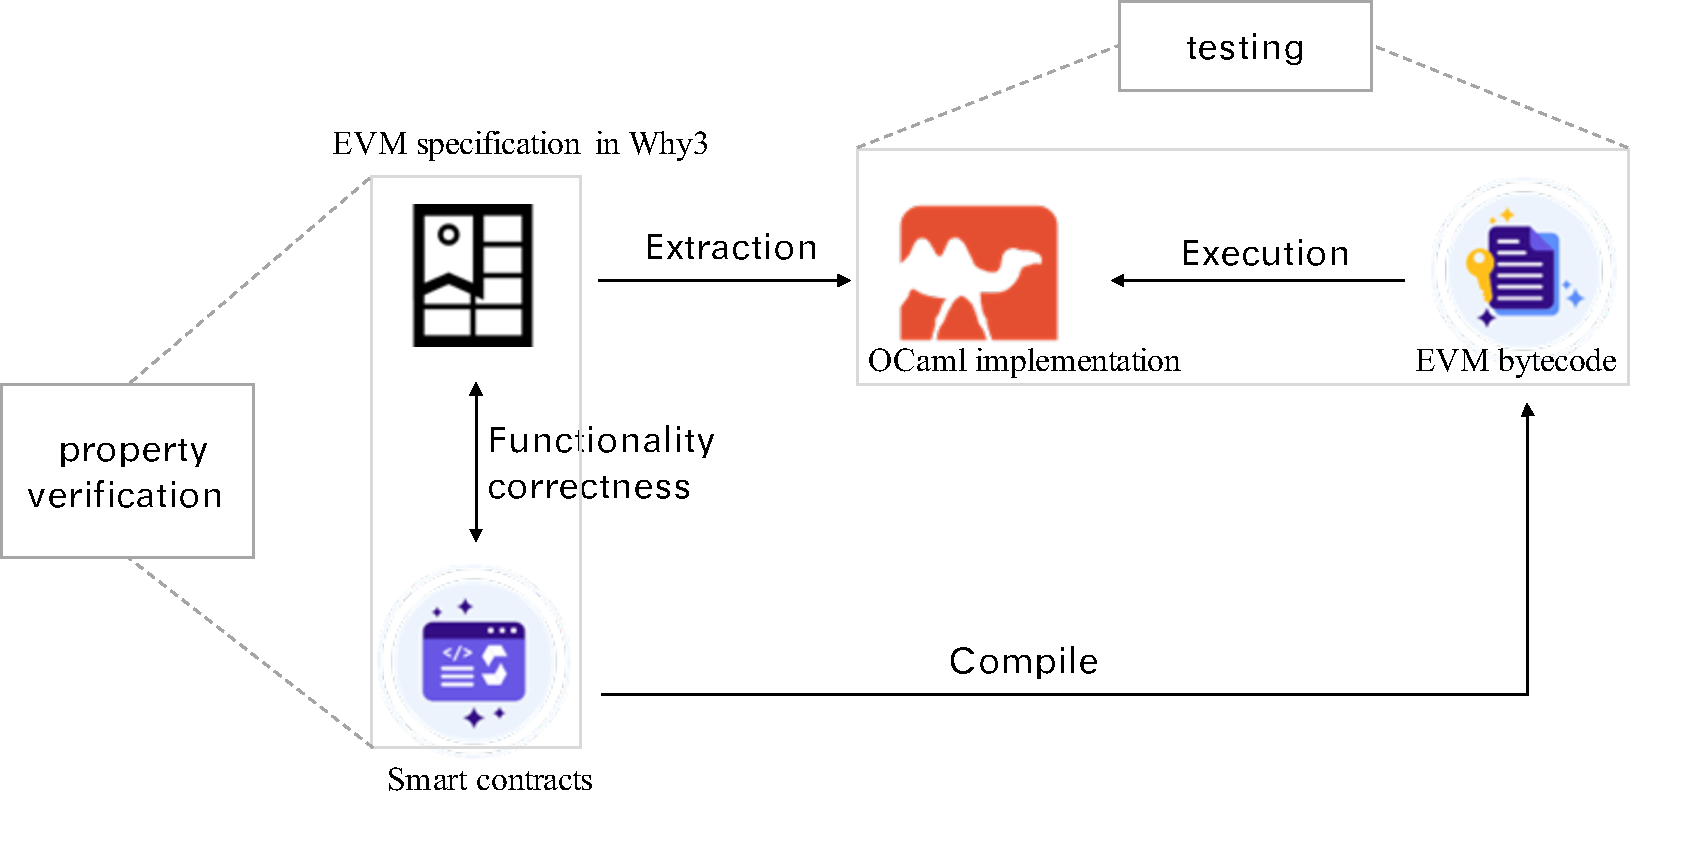
\includegraphics[scale=0.4]{framework.pdf}
  \caption{the Framework of Generating Verified EVM for Production Environment}
  \label{fig:evm1}
\end{figure*}

\section{The Framework of Generating Verified EVM for Production Environment}\label{Sec: Framework}
%\subsection{Methodology of EVM Framework}
In this section, we present the framework of generating verified EVM for production environment in detail. The framework is as shown in Fig. \ref{fig:evm1} and the main idea is to combine verification and testing techniques towards developing secure EVM implementations.
It also provides the potential to verify smart contracts at the bytecode level.  This framework is mainly comprised of two parts: EVM specification in Why3 and experimental testing based on OCaml Extraction and Rust connection. This approach leverages on formal methods and engineering approaches, allowing us to perform both rigorous verification and efficient testing for EVM implementations and further smart contracts. 

\subsection{EVM in Why3}
The first phase of the framework is to define a formal specification of EVM in Why3 and provide a platform for rigorous verification.  
We develop the EVM specification, following the Ethereum project yellow paper~\cite{wood2014ethereum}. More specifically, the EVM implementation is translated into WhyML, the programming and specification language of Why3. %Towards the verification, 
Verification conditions can be further generated through Why3 based on the EVM and property specification. The verification goals can be split into a set of subgoals or directly be proved through the supported Satisfiability Modulo Theories (SMT) solvers. In cases when the automatic SMT solvers cannot deal with, users can resort to interactive theorem provers based on the files generated by Why3.

EVM is essentially a simple stack-based machine. The memory model of EVM is a word-addressed byte array, which is volatile. The storage model of EVM is a non-volatile word-addressed word array. These three components form the infrastructure of EVM. Based on the formalization of the infrastructure, the most important aspect in this framework is to capture the execution result of the EVM instructions. The perspective from which we deal with the execution process of a sequence of opcodes (instructions) is as a state transition process. This process starts with an initial state and leads to a series of changes in the stack, memory etc. The formalization of base infrastructure and the instruction set are specified through \textit{Type Definition} and \textit{Instruction Definition}, respectively. And the \textit{Interpreter Definition} provides the specification of the interpreter and auxiliary functions. 

\subsubsection{Type Definition}\label{sec:type}

To formalize the infrastructure of EVM, we need to first provide the formalization of commonly-used types in EVM, such as the types of machine words and the addresses in the EVM. Hence, we developed a series of type modules such as \texttt{UInt256} and \texttt{UInt160} to ease the representation of corresponding types in EVM. Type alias supported by Why3 are also used to make the basic formalization more readable and consistent with the original definition. 

To this end, the components of the base infrastructure can be easily specified. Stack is defined as a list of elements whose type is \texttt{uint256}, aliased by \texttt{machine word}. Memory is defined as a function that maps \texttt{machine word} to an option type \texttt{option memory\_content}. Since the memory content could be accessed through 256-bit store and 8-bit store instructions, \texttt{memory\_content} is defined as an enumeration type including \texttt{Item8} and \texttt{Item256}. Similarly, storage is defined as a function that maps \texttt{machine word} to \texttt{machine word}. To reflect the implicit change of the machine state, we defined more miscellaneous types. For example, we use \texttt{vmstatus}, \texttt{error} and \texttt{return\_type} to capture the virtual machine status, the operation error, and the view of the returned result. Furthermore, the record type \texttt{machine\_state} is defined to represent the overall machine state which consists of stack, memory, program counter, vmstatus, the instruction list, etc.

\subsubsection{Instruction Definition}\label{sec:instruction}
The infrastructure has been built to specify the state of the virtual machine. %Here we present the formal specification of the action set, i.e., the instruction set. 
Inspired by the instruction formalization in Lem~\cite{hirai2017defining}, the instruction set is defined in multiple groups, such as {\em arithmetic operations} and {\em stack operations}, then these groups are integrated into a summarized type definition \texttt{instruction}. %The definition of \texttt{instruction} is presented as follows, where 
Different subsets of instructions are wrapped up to form the complete specification in the definition of \texttt{instruction}.
\CUT{
\begin{verbatim}
type instruction =
  | Invalid byte
  | Arith arith_inst  
  | Sarith sign_arith_inst
  | Bits bits_inst
  | Info info_inst
  | Memory memory_inst
  | Storage storage_inst
  | Pc pc_inst
  | Stack stack_inst
  | Dup dup_inst
  | Swap swap_inst
  | Log log_inst
  | System system_inst
\end{verbatim}
}

The organization of the instruction category is a bit different from the yellow paper~\cite{wood2014ethereum}. The comparison operations are grouped in the arithmetic operation set \texttt{Arith}; and the comparison operations for signed arithmetic are included in the signed arithmetic operation set \texttt{Sarith}. The bitwise operations and operation \texttt{BYTE} are categorized into the bit-related instruction group \texttt{Bits}. The information related instructions including environmental and block information ones are defined in type \texttt{info\_inst}, except \texttt{CALL} and \texttt{CODE} instructions, such as \texttt{CALLDATACOPY}, \texttt{CODECOPY} and \texttt{CALLDATALOAD}. These instructions are more closely related to memory and stack status. Therefore, extra instructions but closely-related ones are added to the original memory and stack instruction groups. % presented in the yellow paper. 
In case when some illegal command occurs, the instruction \texttt{Invalid} is included in the \texttt{instruction} definition. The \texttt{STOP} operation and the system operations from the yellow paper are defined in the \texttt{System} instruction set. The specification of the remaining instruction groups are basically the same as the corresponding instruction subsets in \cite{wood2014ethereum}. 

\subsubsection{Interpreter Definition}\label{sec:interpreter}
The specification of \texttt{interpreter} formalizes the state transition result of different instructions. For a specific instruction, the interpreter determines the resultant machine status developing from the current status. Some auxiliary functions are defined
to make the definition of the interpreter more concise and compact. For example, the following function is used to obtain the next instruction to be executed. It is obtained from the instruction list following the program counter. 
\begin{verbatim}
let get_inst (mac_st: machine_state): option instruction =
  match mac_st.mac_pc, mac_st.mac_insts with 
  | pc, insts -> (nth pc insts) 
  end    
\end{verbatim}

Pop and push operations are the most commonly-used manipulations for the state transition of stack. Auxiliary functions \texttt{push\_stack} and \texttt{pop\_stack} are defined to control the change of stack status. For capturing the status transition result of \texttt{Swap} instructions, recursive functions \texttt{fetch} and \texttt{drop} are defined to support more direct manipulation on lists. Another function \texttt{swap\_stack} is defined further for state transition of swap instructions.
With these pre-defined auxiliary functions, the definition of the interpreter function is essentially comprised of machine status update with regard to concrete instructions. 

\begin{figure*}[t]
  \centering
  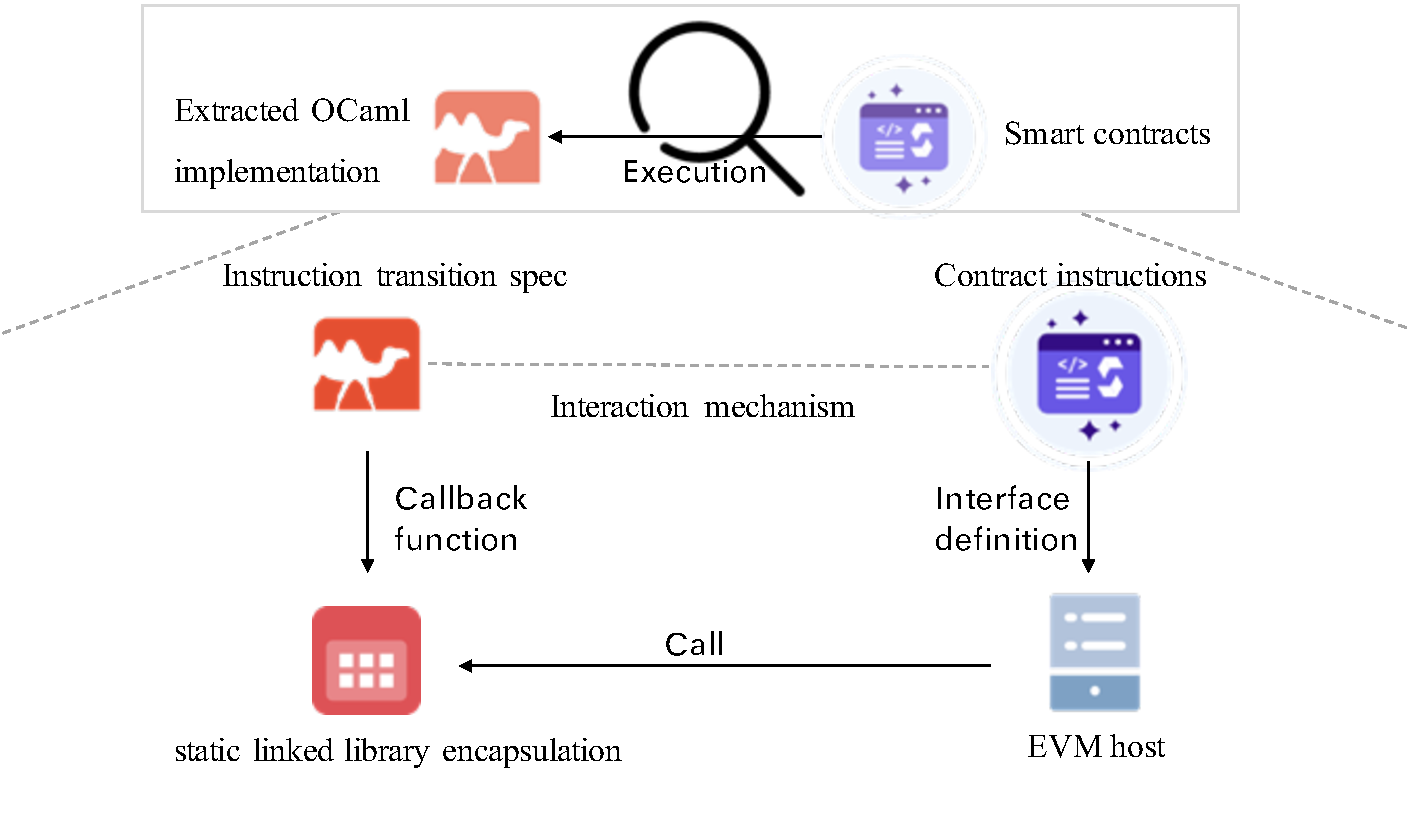
\includegraphics[scale=0.4]{runninginPE.pdf}
  \caption{Running EVM in Production Environment}
   \label{fig2}
\end{figure*}

\subsection{Running EVM in Production Environment}
%We customizedly defined a series of drivers to %extract WhyML programs into OCaml programs. 
Fig. \ref{fig2} shows the second phase of the framework: deploy the verified EVM, encoded in Why3, in production environments. The deployment is essentially based on a co-compilation framework between OCaml and Rust.

OCaml is a functional programming language where the programs can be compiled either to OCaml bytecode or executable binaries. In the latter case, a runtime library is attached to handle various non-functional features like memory management. Through the \texttt{Callback} module, OCaml allows us to register a set of callback functions which can be used as an interface in static or dynamic linking. 
So we first defined a series of customized drivers to extract WhyML programs into OCaml programs. After the extraction, the OCaml implementation of EVM is then encapsulated and exposed as a static linked library. This library can be further called by the EVM host in Rust.

Rust is a multi-paradigm system programming language which is designed to provide better memory safety while maintaining high performance \cite{LBHN16}.
The framework provides the interaction mechanism between Rust and Why3. By gluing them together, verified models can be directly executed in production environments for further testing. The coupling between Rust and extracted OCaml implementation enables us to perform VM tests to test the basic workings of the verified VM. Information of the overarching environment is obtained through the interface of Rust implementation, and the test can be performed on the execution of the OCaml implementations to check the operations in different transactions.    

\subsection{Examples of Property Verification and Tests}

We now show some examples of property verification towards smart contracts and tests against Ethereum 
test suites. Specifically, we present the specification and verification of \emph{SafeMath} library and \emph{SimpleAuction} contract.
For the tests, we perform the testing of arithmatic operations against the Ethereum test suite.

\paragraph{Overflow/Underflow property verification.}
We first take the example of \emph{SafeMath} from Solidity 
library. Overflow/Underflow problems often occur when we deal with number operations. For EVM, the unsigned integer type we 
perform arithmatic operations on range from 0 to $2^{256}$, which is specified as \texttt{uint256} in the WhyML specification.
The properties we verify are to guarantee that overflow and underflow problems would not occur in the number operations.
Besides, the correctness of the operation results is also specified in the postconditions and further verified, for example,
the last postcondition in the function \texttt{div\_safe}. 

As can be seen from the following definition of \texttt{div\_safe},
the function body is comprised of three parts, as a Hoare triple, 
preconditions, program expressions and postconditions.
The first precondition specifies that the divisor should be greater than
zero. The first postcondition states that the returned value should
satisfy the required property with no underflow issues. The other
two postconditions are to guarantee the correctness of the operation result. 
\begin{verbatim}
let div_safe (a:uint256) (b:uint256): uint256
requires {to_int b > 0}
ensures {to_int result >= 0}
ensures {to_int a = 0 -> to_int result = 0}
ensures {to_int a <> 0 -> 
to_int a = (to_int result) * (to_int b) + mod (to_int a) (to_int b)}
= a / b
\end{verbatim}

We now proceed to the verification of the properties. The verification conditions can be obtained 
through running \texttt{why3 prove} on the WhyML file. 
The proving goals for \texttt{div\_safe} are derived as follows:

\begin{verbatim}
goal VC div_safe :
forall a:uint256, b:uint256.
  to_int b > 0 -> (not b = 0 && in_bounds (div a b)) /\
  (forall result:uint256. result = div a b -> to_int result >= 0 &&
  (to_int a = 0 -> to_int result = 0) &&
  (not to_int a = 0 ->
  to_int a = (to_int result * to_int b + mod (to_int a) (to_int b))))
\end{verbatim}
To prove the goals, we first apply the \texttt{split VC} transformation and 
then call theorem provers \emph{alt-ergo} and \emph{cvc4} 
to prove the subgoals automatically. The proof session state will be 
stored in an XML file, which includes the proved WhyML file, the applied
transformations, the used provers and the proof results.
Complete proving goals derived from the functions and 
proof sessions can be found at \cite{Examples}.
%\url{https://github.com/Xiyue-Selina/coordination20}.

\paragraph{Open Auction contract verification.}
The open auction contract is mainly comprised of three functions:
(1)~Everyone can send their bids through the \texttt{bid} function when the bidding period is not finished.
When the bid sent by one bidder exceed the current recorded highest bid, the auction state including the highestBidder and highestBid would be updated. Then the withdrawal amount of the previous
highest bidder should be increased by the previous highest bid.
(2)~When one bid is beat by another higher raised bid, the previous bid should be returned back to the
corresponding bidder. Bidders can call the \texttt{withdraw} function to get the money/Ether back.
(3)~The auction is ended by the \texttt{auctionEnd} function. If current time is over the auctionEndTime,
then the auction \texttt{end\_state} should be set to True. As the bidding ended, the beneficiary would 
receive the final highest Bid.

In the WhyML specification, \texttt{auction\_status} records the current state of the auction including the current 
highest bidder, the highest bid and the auction ended state. \texttt{auction\_constant} records the beneficiary and the
auctionEndTime and \texttt{auction\_ended} records the final bidder, bid and the beneficiary claimed money/Ether amount.
The properties to be verified are to guarantee the correctness of the functionality. For example,
in the \texttt{auctionEnd} definition, the postcondition specifies the constraints of 
auction ended state and beneficiary claimed amount that the returned result should satisfy.
Complete specification of the three functions can be found at \cite{Examples}.
%\url{https://github.com/Xiyue-Selina/coordination20}. 
The generated verification conditions can be discharged through \emph{alt-ergo} and \emph{cvc4} automatically.

\begin{verbatim}
let auctionEnd (current_time: uint) (auc_st: auction_status) 
(auc_const: auction_constant) (auc_end: auction_ended): 
(auction_status, auction_ended) 
... ensures {let (_auc_st, _auc_end) = result in 
_auc_st.end_state = True 
&& _auc_end.finalBidder = auc_st.highestBidder 
&& _auc_end.finalBid = auc_st.highestBid
&& _auc_end.bene_amount.benefici = auc_const.beneficiary 
&& _auc_end.bene_amount.benefit_amount = _auc_end.finalBid} = ...
\end{verbatim}

\section{Related Work}\label{Sec: Related}

Research interest of blockchain technology has exploded since the inception of Bitcoin. As the popularity of the second generation of blockchain, 
Ethereum, grows, a series of security vulnerabilities have also appeared. 
Since EVM and smart contracts deal directly with the transactions of valuable cryptocurrency units among multiple parties, 
the security of smart contracts and EVM implementations is of paramount importance. To address the security challenges, 
researchers resorted to the techniques of formal methods and program analysis. 

%\begin{itemize}
%    \item \textbf{Formalization Foundation of EVM} 
\noindent\textbf{Specification and Verification.}~An executable formal semantics of EVM has been 
created in the K framework by Everett et al.~\cite{hildenbrandt2017kevm}. 
Compared with KEVM with the support
of matching logic for verification, we use Hoare logic, which serves as a good framework for
verification condition specification, to avoid the complex definitions
of the operational semantics. 
A framework to analyze and verify both the runtime safety and the functional correctness of 
Solidity smart contracts in F*
% , a functional programming language aimed at program verification,
was presented in \cite{bhargavan2016formal}.
Hirai~\cite{hirai2017defining} proposed an EVM implementation in Lem, a language that can be compiled for 
a few interactive theorem provers. Then, safety properties of smart contracts can be proved in proof assistants like Isabelle/HOL.
While in our work, we use WhyML for specification and programming, which supports both logical theories 
and programming data structures. Moreover, both automated and interactive external theorem provers 
can be relied on to discharge verification conditions. 
% Generally, the central design choice of the framework is to leverage the infrastructure of 
% Why3, the deductive verification platform where a set of external theorem provers, both automated and interactive, 
% can be relied on to discharge verification conditions. At the same time, 
% OCaml programs can be directly extracted from WhyML programs through the extraction mechanism for further tests.
% Besides the above formalizations of EVM, 
% there are also implementations of EVM in other languages such as %Javascript~\cite{vmjs}, 
% Go~\cite{vmgo} and Ruby~\cite{cryptape}.
%    \item \textbf{Verification of Smart Contracts} 

\noindent\textbf{Testing and Debugging.}~The \texttt{hevm} project~\cite{hevm} is implemented in Haskell for unit testing and debugging of smart contracts.
% though the EVM implementation is not completed yet. 
Sergey et al.~\cite{sergey2017concurrent} provided a new perspective between smart contracts and concurrent objects,
 based on which existing tools and insights for understanding, 
 debugging and verifying concurrent objects can be used on smart contract behaviors. 
 In \cite{luu2016making}, several new security problems were pointed out and a way to enhance the operational semantics of 
 Ethereum was proposed to make smart contracts less vulnerable. 
 Due to the difficulty of correcting the semantics of Ethereum, Luu et al.
 ~\cite{luu2016making} also implemented a symbolic execution tool \texttt{OYENTE} to find security bugs.
While in our work, executable OCaml programs can be directly extracted from WhyML programs for further tests 
with the support of extraction mechanism.
%  of the deductive verification platform.
 
%\end{itemize} 

\section{Conclusion}\label{Sec: Conclusion}
We propose a framework to enable formal specification, verification and testing towards EVM. In this framework, the formalization of EVM is specified in WhyML, the programming and specification language of Why3. Based on the EVM formalization, automatic SMT solvers and interactive theorem provers provided in Why3 can be employed for verification. The OCaml implementation of EVM is extracted from the WhyML specification and then glued with Rust implementation based on the coupling framework. The coupling framework provides the interaction mechanism between OCaml and Rust, which allows us to perform tests on the new implementation without additional interface implementation.

\subsection*{Acknowledgement}
\noindent This work has been supported by the National Natural Science Foundation of China under grant no. 61772038 and 61532019, and the Guangdong Science and Technology Department (Grant no.2018B010107004). Thanks to members of Cryptape, especially Jan and Zhiwei, for the helpful discussions during the development of this framework.


\bibliographystyle{splncs04}
\bibliography{the}

\end{document}

